% Appendix B

% variables
\newcommand{\appdirb}{appendices/plots/appendixB}

\chapter{Physics tool}

\label{AppendixB}

\section{Synchrotron radiation}
\label{appB:sec:sr}

Synchrotron radiation is the known phenomenon based on the basic principle of the electrodynamics, which states that an accelerated charged particle always radiates electromagnetic waves. In particular, synchrotron radiation describes the energy emitted by a charged particle in a circular motion. This phenomenon was already investigated theoretically at the beginning of the 20th century and was later first observed and experimentally studied at the General electric 70 MeV synchrotron from which it gets its name \cite{synchrotron-radiation}. \\
This type of radiation is well-known thanks to the advent of modern circular accelerators, where it is so strong that it can even be observed for heavy particles, for instance protons. \\
In NA64 this radiation is used to tag the incoming particles to distinguish between the electron primaries and the background given by hadrons and muons. A small review of this effect, which will underline the important properties exploited for the experiment, will be presented.


\subsection{Power emitted}
The first result about the power radiated by an accelerated non-relativistic particle was obtained by Larmor:

\begin{equation}
S = \frac{e^2}{6 \pi \epsilon_0 m_0^2 c^3}\left(\frac{dp}{dt}\right)^2
\label{eqn:radiated-power}
\end{equation}

The angular distribution can be calculated similarly:

\begin{equation}
\frac{dS}{d\Omega} = \frac{e^2}{(4 \pi)^2 \epsilon_0 m_0^2 c^3}\left(\frac{dp}{dt}\right)^2\sin^2\Theta
\label{eqn:angular-dist}
\end{equation}

where $d\Omega = \sin{\Theta} d\Theta d\phi$. If we insert the numbers in the two previous equations it results that the power irradiated for a particle in the classical approximation is negligible even for particles as light as the electrons.

The situation changes as we try to find a Lorentz-invariant form of the equation by applying the following transformation:
\begin{eqnarray}
dt \longrightarrow d\tau=\frac{1}{\gamma}dt \qquad
\gamma = \frac{1}{\sqrt{1-\beta^2}} \qquad \beta=\frac{v}{c}
\label{time_trans}
\end{eqnarray}

\begin{equation}
\left(\frac{dP_{\mu}}{d\tau}\right)^2 \longrightarrow \left(\frac{dp}{dt}\right)^2 - \frac{1}{c^2}\left(\frac{dE}{d\tau}\right)^2
\label{momentum-trans}
\end{equation}

If we put these expressions in Eq.\ref{eqn:radiated-power} we get a correspondent relativistic expression:
\begin{equation}
S = \frac{e^2c}{6\pi \epsilon_0}\frac{1}{(m_0c^2)^2 }\left[\left(\frac{dp}{dt}\right)^2 - \frac{1}{c^2}\left(\frac{dE}{d\tau}\right)\right]
\label{eqn:rel-power}
\end{equation}

The acceleration will strongly depend on the angle between the particle velocity and the acceleration as the time derivate of the impulse suggests. We will now concentrate on the extreme case where $dv/dt \perp v$ since it is our case of interest. It is possible, however, to derive the other extreme case $dv/dt~||~v$ and verify that there is no difference from the classical one. \par

If we assume the particle to follow a circular motion (i.e $F \perp v$) we can conclude that the energy of the particle does not change during the motion. This already drops out the time-derivative of the energy from Eq.\ref{eqn:rel-power}. After that, we can express the momentum of the particle as:
\[\frac{dp}{dt} =p\omega = p \frac{v}{R}\]
where R is the bending radius of the trajectory. We can further simplify the expression assuming $E=pc$, which is true for a particle at high enough energy and it is certainly true for our experiment where the electrons have an energy of 100 GeV. After we express the momentum and velocity using these last approximation we get the result of:
\begin{equation}
S = \frac{e^2c}{6\pi \epsilon_0}\frac{1}{(m_0c^2)^4 }\frac{E^4}{R^2}
\end{equation}

Normally the power is integrated through a circle to calculate the energy emitted per full turn:

\begin{equation}
\Delta E = \oint S dt = \frac{e^2}{3\epsilon_0(mc^2)^4}\frac{E^4}{R}
\label{eqn:energy-emitted}
\end{equation}

For a very energetic electron ($\gamma >> 1$) we can reduce the above result to a compact formula particularly useful to plug-in the numbers and that is valid in the condition of our experiment:

\begin{equation}
\Delta E[keV] = 88.5\frac{E^4[GeV]}{R[m]}
\label{eqn:energy-emitted-simp}
\end{equation}

In the NA64 experiment, this is not entirely the case since the particle will be under the influence of the magnetic field only for 2-4 \si{\meter}. However, because of the radial symmetry, a factor $l/2\pi R$ (where $l$ is the portion of the circle inside the magnetic field) is sufficient to correct the equation. Eq.\ref{eqn:energy-emitted} already contains all the scaling and the physics we are interested in.
 Since for constant magnetic field, $R$ is constant too, there are only two scalings that are significant in Eq.\ref{eqn:energy-emitted}:
 \begin{enumerate}
 \item An inverse scaling to the fourth power of the mass. This means that heavy particles will produce much less radiation, in particular $\mu^{+/-}$ and $\pi^{+/-}$ that have a mass approximately 200 times the one of the electron will irradiate 5$\times 10^{-8}$ times less. This very high suppression factor is however reduced in our experiment since it is still possible for a heavy particle to ionize electrons and give them enough kinetic energy to leave a synchrotron-like signal in the detector. For particles heavier than the electron the maximum energy exchanged in a collision is 1 GeV, the cross-section of such interactions can be safely approximated by the Rutherford differential cross-section at these energies and it roughly depends on the inverse of the energy transferred to the ionized electrons \cite{review-particle-physics}. The simulation estimates such interactions to happen with a probability of $\sim 10^{-4}$ for 1 MeV transferred energy (enough to leave a fake signal in the detector). Therefore, they dominate the value of the suppression factor.
 \item A scaling with the energy to the fourth power. This would make it possible to correlate the deposited energy in the detector with the momentum of the particle. There are however several problems that limit this approach, like the overlap of the synchrotron radiation spectra (see Fig.\ref{fig:synch_spectrum}), as well as the possibility for an electron interacting with some material or with residual gas to emit photons via Bremsstrahlung. We conclude that such an approach is not feasible to achieve the sensitivity required by our experiment and therefore synchrotron detectors are no substitute to a more efficient tracking system.
 \end{enumerate}
 
 \subsection{Radiation angular distribution}
 To calculate the angular distribution of the photon emitted we can, for simplicity, consider the extreme case where the photons are ejected perpendicular to the particle motion in the center of mass system. The $\sin^2 \theta $ scaling in Eq.\ref{eqn:angular-dist} tells us that these photons will represent the maximum intensity.\\
 If we assume $z$ to be the direction of motion and the photon to be emitted in the perpendicular direction $y$ we can apply a Lorentz boost in the z-direction to check the photon emission in the laboratory system:
 \[
 p_0 = 
 \begin{pmatrix}
 p_y \\ 
 0
 \end{pmatrix}
\longrightarrow
p_0'=
\begin{pmatrix}
p_y \\
\gamma \beta p_y 
\end{pmatrix}  
 \]

Where $p_y$ is the momentum of the photon in the center of mass system. \\
This means that the angle between the momentum of the particle and the one of the photon will be:
\begin{equation}
\tan \Psi = \frac{p_y}{\gamma \beta p_y} \Rightarrow \Psi \sim \frac{1}{\gamma} \qquad (\gamma >> 1)
\end{equation}

For a typical 100 GeV e$^-$ this angle would be $\sim$ $10^{-5}$ radian. Thus, to assume that the photons are emitted parallel to the particle motion direction for such energies is a good approximation.

\subsection{Radiation spectrum}
The relativistic electron moving along the orbit produces at the observer position an electromagnetic pulse of length $t_{pulse}$. In the previous approximation for small emission angles, we can calculate this time as the difference between the photon and electron time of flight as the electron travels along the arc drawn by this angle $\Psi$:
\[t_{pulse} = t_e - t_{\gamma} =  \frac{2R\Psi}{c \beta} - \frac{2 R \sin \Psi}{c}
\approx \frac{2R}{c}\left(\frac{\Psi}{\beta}-\Psi+\frac{\Psi^3}{3!}+\cdots\right)
\]

at high energy we can safely use the approximation of $\beta \gamma \sim \gamma - 1/2\gamma$ and $\Psi \sim 1/\gamma$:
\[t_{pulse} \approx \frac{2 R}{\gamma^3 6c}\]

This short impulse will generate a broad impulse with a typical radiation frequency of:
\[\omega_{typ} \approx \frac{2 \pi}{t_{pulse}} \approx \frac{3 \pi  c \gamma^3}{2 R} \]

The spectral function of such a photon can be described using \cite{synchrotron-radiation}:
\begin{equation}
\label{eqn:sync_spectrum}
S_s(\xi) = \frac{9 \sqrt{3}}{8 \pi}\xi \int_{\xi}^{\infty}K_{5/3}(\xi)d\xi
\end{equation}
where we define $\xi = \omega/\omega_c$ given the \textbf{critical frequency} $\omega_c =\omega_{typ}/\pi$ which divides the spectrum in two parts of equal power. This same spectrum was observed in the MC simulation (Fig.\ref{fig:synch_spectrum}), however when we include the Bremsstrahlung interactions the spectra is dominated by it and it becomes impossible to distinguish electrons of different energy as as one would assume just by looking at the scaling in Eq.\ref{eqn:energy-emitted}.


\begin{figure}[h!]
\centering
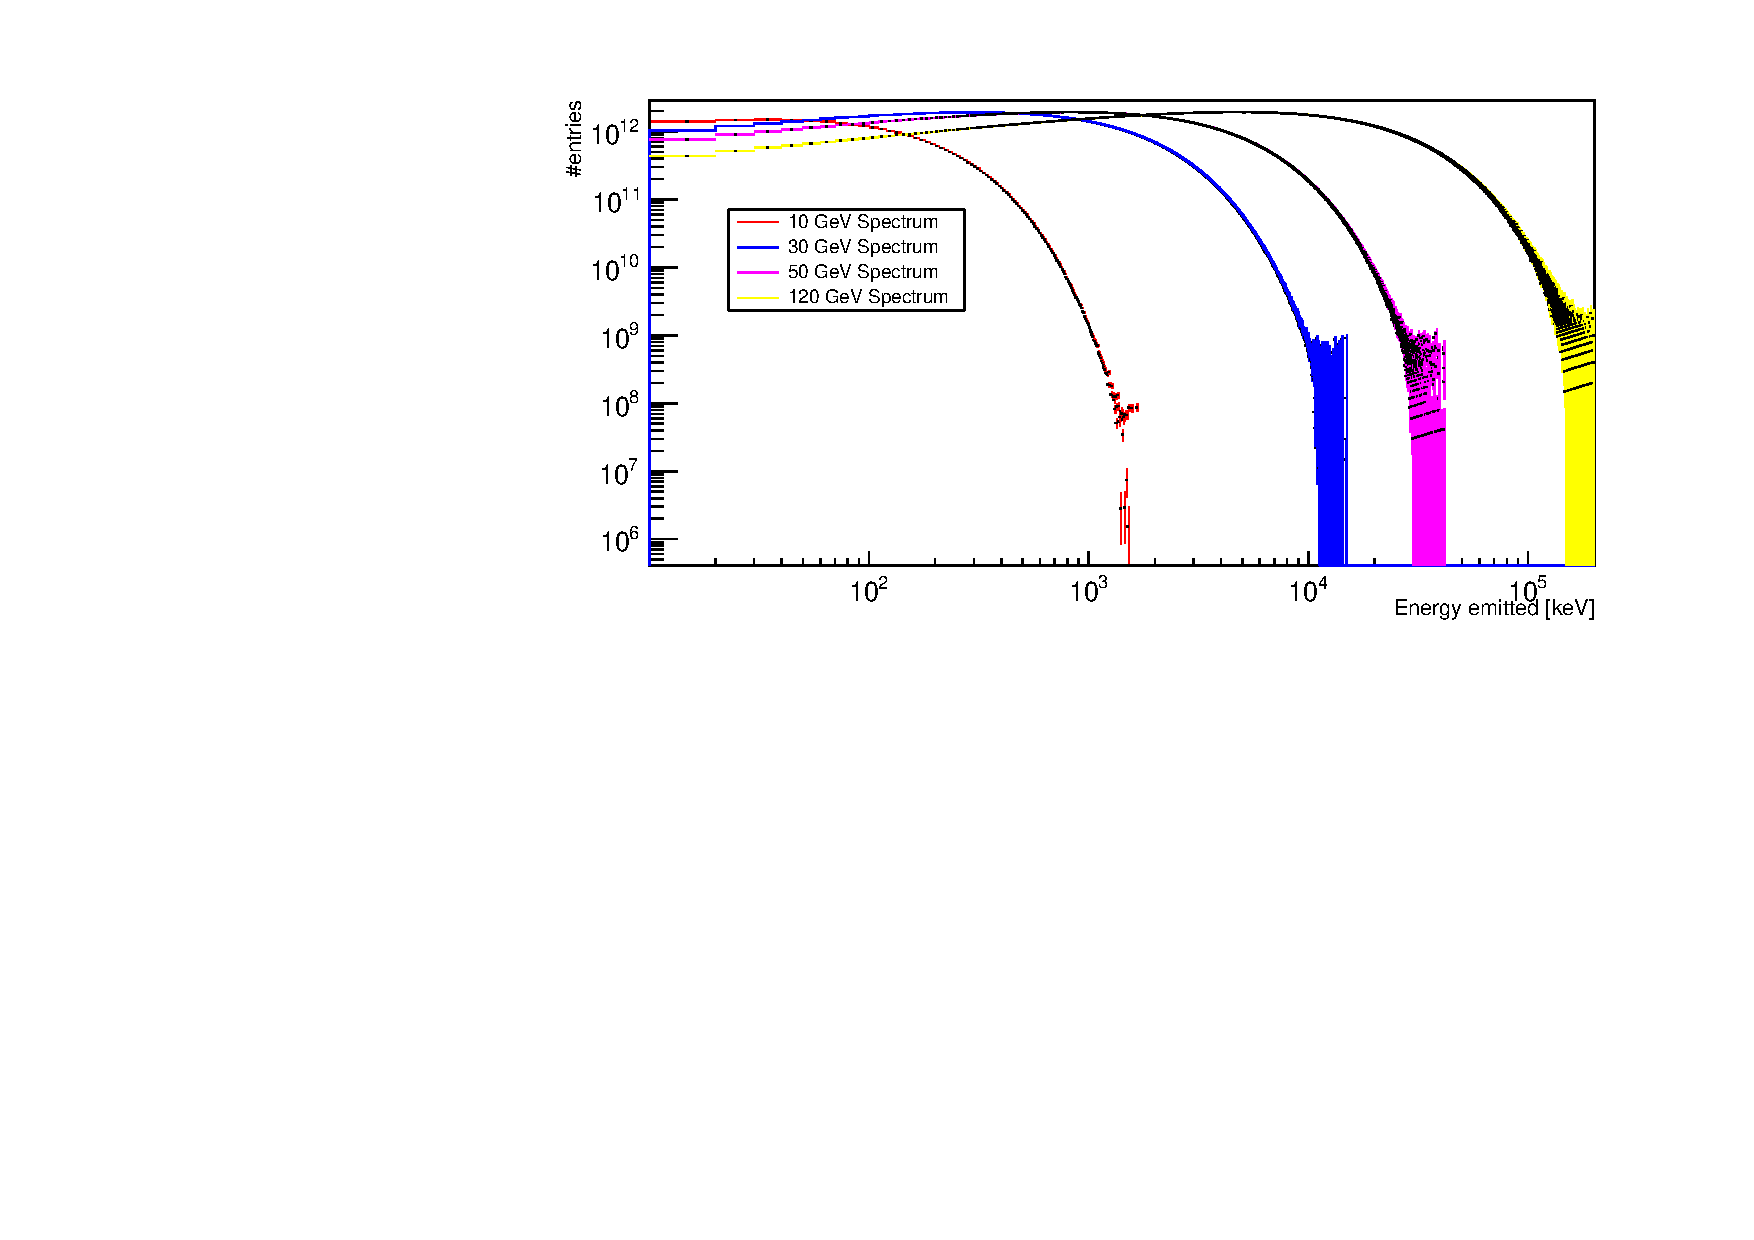
\includegraphics[width=\textwidth,height=0.55\textwidth]{\appdirb/syn_spectra.pdf}
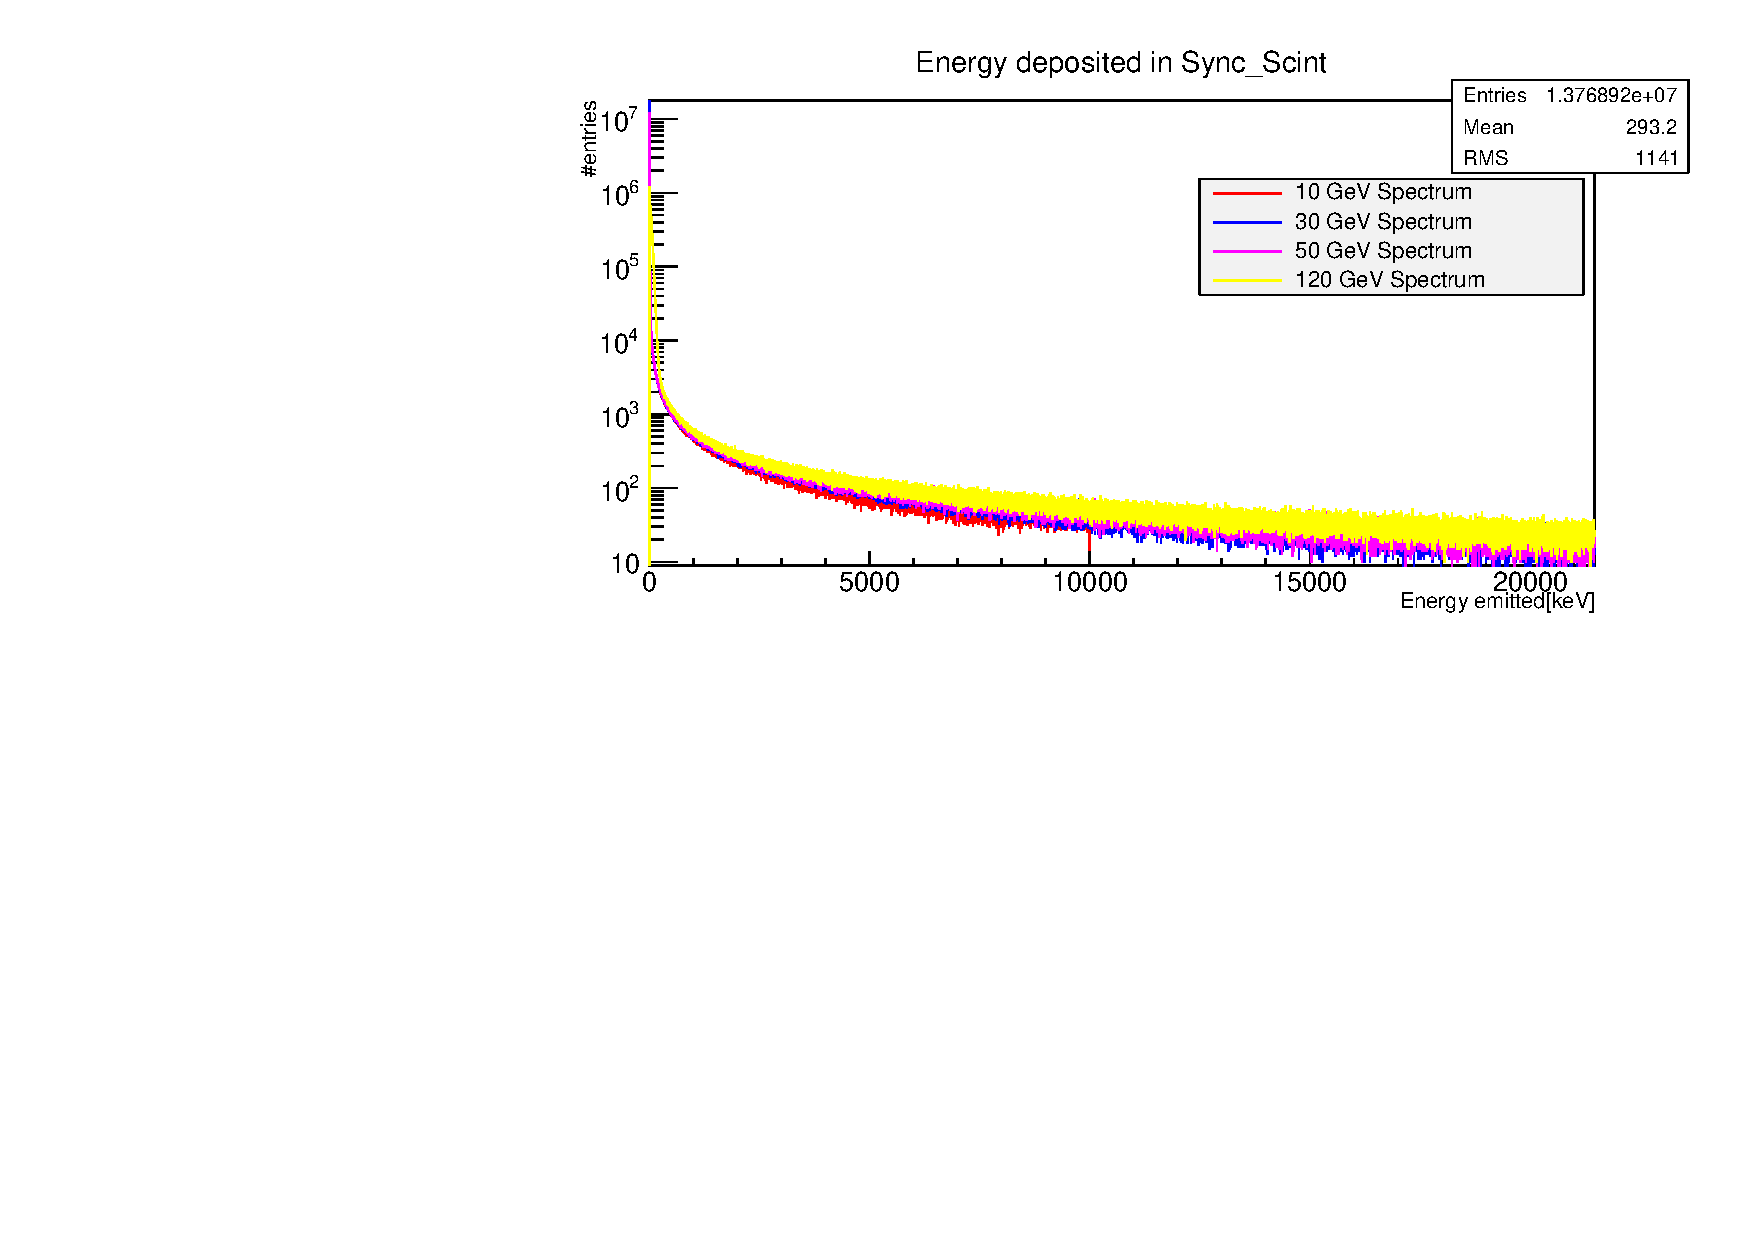
\includegraphics[width=\textwidth,height=0.55\textwidth]{\appdirb/brems_spectra.pdf}
\caption{Upper plot: Spectrum for a single synchrotron radiation photon emitted by an electron in the MC simulation. \\
Bottom plot: Total energy deposited in the BGO for one electron event after Bremsstrahlung is included in the simulation.}
\label{fig:synch_spectrum}
\end{figure}

\FloatBarrier\noindent
\section{Profile construction for shower profile analysis}
\label{Appb:sec:make_profile}

A shower profile database can be understood as an $N\times N$ matrix
where each entry represents a portion of the ECAL cell of dimension
$d_x \times d_y$. Each entry of the matrix contains the mean value of
energy deposited in the cell when the incoming particle hits the
portion of the ECAL plane described by that entry. To also
account for the deviation that such a shower can have as a function of the
hitting point one would need a second matrix to encode such
information. To build such database the root class \textit{TProfile2D} was used \cite{root-tprofile}.

The main parameters that play a role in the construction of the shower
profiles are the dimensions of the area that is covered by the
\textit{TProfile2D}, and the dimensions $d_x \times d_y$ that each bin has,
which represents the minimal distance between two hit points resolvable by the database.  The total dimension that the profile
should have can be trivially set to be equal to the ones of one ECAL
cell (38.2$\times$38.2 \mms) since our cuts already require the majority of the shower to be contained in the cell aligned with the beam spot. The problem of the bin dimension is
more subtle: due to the shower symmetry there is no particular reason
to set $d_x \neq d_y$ the precise dimensions of the bin must be a
compromise between having a large bin that allows good statistic and a
small bin that allows enough precision. The large sample of electrons
collected in NA64 typically allows good statistics for each bin even
when their dimension is below 1 $\mmi$. However, defining a bin smaller
than the accuracy achievable in the extrapolation of the Micromegas line (see Sec.\ref{ch3:sec:bkg-ecal-profile}) to the ECAL should be avoided. This error can be
derived analytically:
\begin{equation}
  \sigma_{ECALxy} = \sigma_{mm}\sqrt{1+2t^2}
  \label{eqn:MMerror}
\end{equation}

\begin{equation}
  t = \frac{Z_{ECAL}-Z_{MM4}}{Z_{MM4}-Z_{MM3}}
  \label{eqn:T}
\end{equation}

where:
\begin{description}
\item[$\sigma_{ECALxy}$]: is the error of the hit position extrapolated to the ECAL in the xy-plane.
\item[$\sigma_{mm}$]: is the resolution of the hit position in each
  Micromegas.
\item[$Z_{MM}$]: Micromegas Z-axis position.
\item[$Z_{ECAL}$]: position in the Z-axis of the ECAL plane.
\end{description}

This results in a resolution of $\sim$130 $\mu$m for our setup. A more
complicated expression was considered to take into account possible
misinformation in the position of the detectors. While the 
entrance angle of the particle was checked to have small effects on
$\sigma_{ECALxy}$, assuming some error on the position of the
detectors increases the error by a factor 2-4 for values around 1-2
\si{\centi\meter}. The work presented here was performed using a TProfile2D
with a bin size of 0.34 $\mmi$ which accounts for such uncertainties.

Electron calibration runs were used to produce the profiles to have a sample of electrons, cuts were applied to reject the contamination caused by the hadrons in the beam and out-of-time energy events. \\
The following criteria were applied for the profiles tested in this note:

\begin{itemize}
\item Single cluster in each Micromegas
\item Energy larger than 1 MeV and smaller than 70 MeV in each SRD
  plane
\item Coincidence of $\sim$1 ns between timing in cell (3,3) of ECAL
  and $S_0$ time.
\item Pedestal fluctuation less than 10 ADC in cell (3,3) and each of
  the surrounding cells.
\end{itemize}

The production of the database is done for the events selected by computing the hit point of the incoming particle in cell
3x3 and updating the value of the corresponding bin in each of the 36
TProfile2D representing each cell. The specific value filled is the
percentage of energy deposited in the cell, i.e. $100 \times E^i/E^{tot}$.

After the profiles are constructed, they can be used to calculate the compatibility of a single event with an em-shower. The algorithm for the $\chi^2$ computation works as follows:
\begin{enumerate}
\item The values of the xy coordinates of the hitting point of the particle are computed by extrapolating to the ECAL position the line passing through the hit point of the last two Micromegas planes.
\item The predicted values $E_{pred}^i$,$\sigma^{i}_{pred}$ are read from the database in the corresponding bin.
\item The values $E_{mes}^i$ are computed normalizing the energy $E^i$ of each cell to the total energy measured in the ECAL.
\item The value of $\chi^2$ is calculated using Eq.\ref{eqn:chi} and is normalized to the number of cells considered.
\end{enumerate}

%%% Local Variables:
%%% mode: latex
%%% TeX-master: "../PhDthesis"
%%% End: